% \documentclass[dvipdfmx, 10.5pt]{beamer}
\documentclass[aspectratio=169, dvipdfmx, 11pt,uplatex]{beamer} % aspectratio=43, 149, 169
\usepackage{here, amsmath, latexsym, amssymb, bm, ascmac, mathtools, multicol, tcolorbox, subfig}
%画像挿入
\usepackage[absolute,overlay]{textpos}
%デザインの選択(省略可)
\usetheme{Luebeck}
%カラーテーマの選択(省略可)
\usecolortheme{orchid}
%フォントテーマの選択(省略可)
\usefonttheme{professionalfonts}
%フレーム内のテーマの選択(省略可)
\useinnertheme{circles}
%フレーム外側のテーマの選択(省略可)
\useoutertheme{infolines}
%しおりの文字化け解消
\usepackage{atbegshi}
\ifnum 42146=\euc"A4A2
\AtBeginShipoutFirst{\special{pdf:tounicode EUC-UCS2}}
\else
\AtBeginShipoutFirst{\special{pdf:tounicode 90ms-RKSJ-UCS2}}
\fi
%ナビゲーションバー非表示
\setbeamertemplate{navigation symbols}{}
%既定をゴシック体に
\renewcommand{\kanjifamilydefault}{\gtdefault}
%タイトル色
\setbeamercolor{title}{fg=structure, bg=}
%フレームタイトル色
\setbeamercolor{frametitle}{fg=structure, bg=}
%スライド番号のみ表示
%\setbeamertemplate{footline}[frame number]
%itemize
\setbeamertemplate{itemize item}{\small\raise0.5pt\hbox{$\bullet$}}
\setbeamertemplate{itemize subitem}{\tiny\raise1.5pt\hbox{$\blacktriangleright$}}
\setbeamertemplate{itemize subsubitem}{\tiny\raise1.5pt\hbox{$\bigstar$}}
% color
\newcommand{\red}[1]{\textcolor{red}{#1}}
\newcommand{\green}[1]{\textcolor{green!40!black}{#1}}
\newcommand{\blue}[1]{\textcolor{blue!80!black}{#1}}

\begin{document}

\begin{frame}{KeTCindyChatの概要}
私たちはKeTCindyのコードを対話形式で生成できる「KeTCindyChat」を開発した。これにより、ユーザーはチャット形式で質問やリクエストを入力し、リアルタイムでKeTCindyのコードを生成することができるようになるだろう。
\begin{textblock*}{0.3\linewidth}(30pt, 150pt)
    \centering
    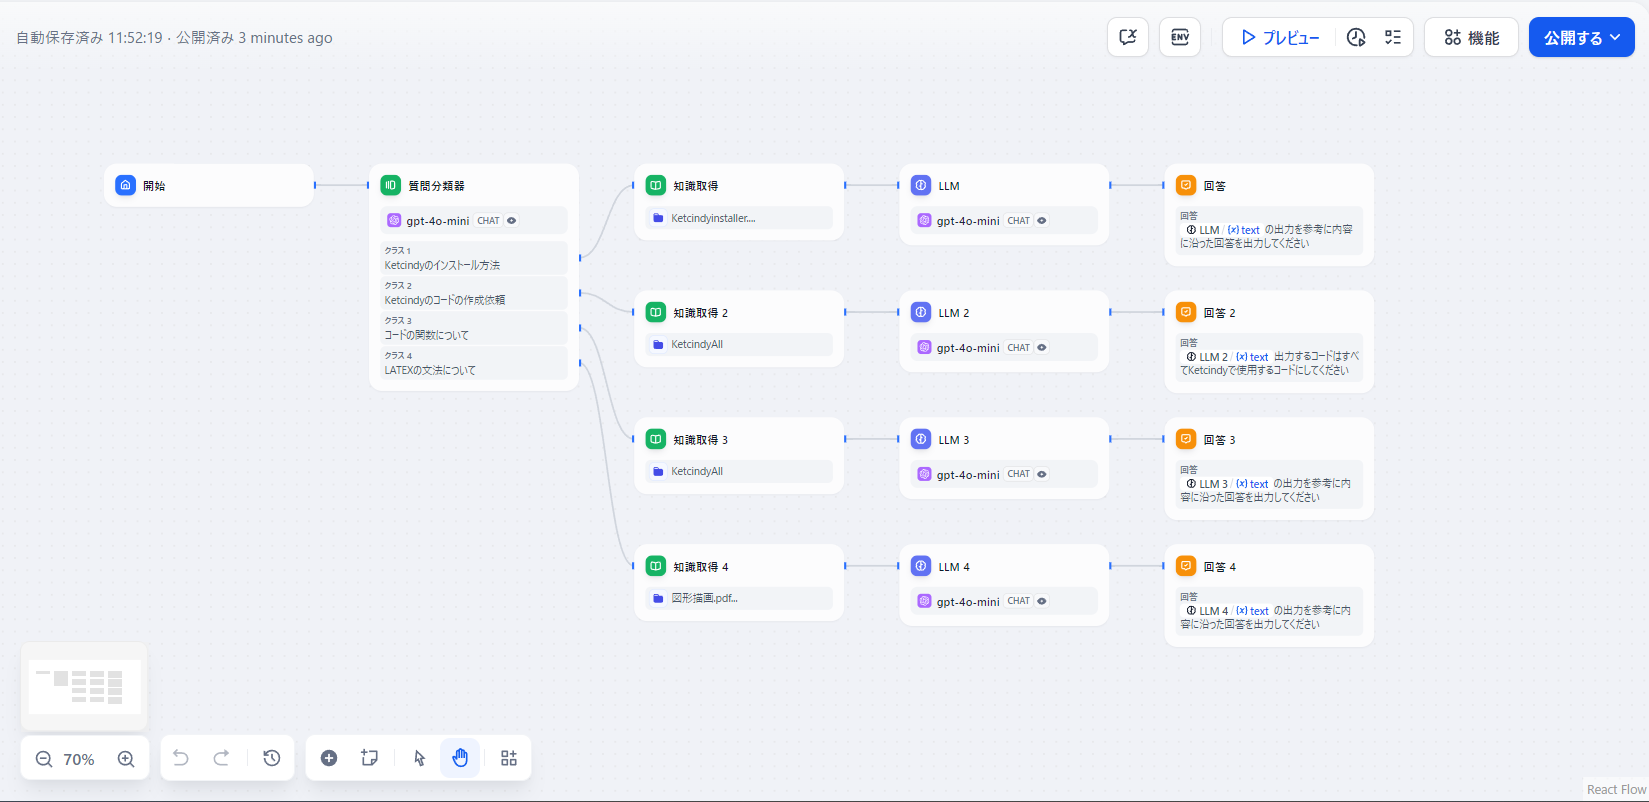
\includegraphics[width=\linewidth]{Chatslide/appabout.png}
  \end{textblock*}
  
  \begin{textblock*}{0.3\linewidth}(170pt, 150pt)
    \centering
    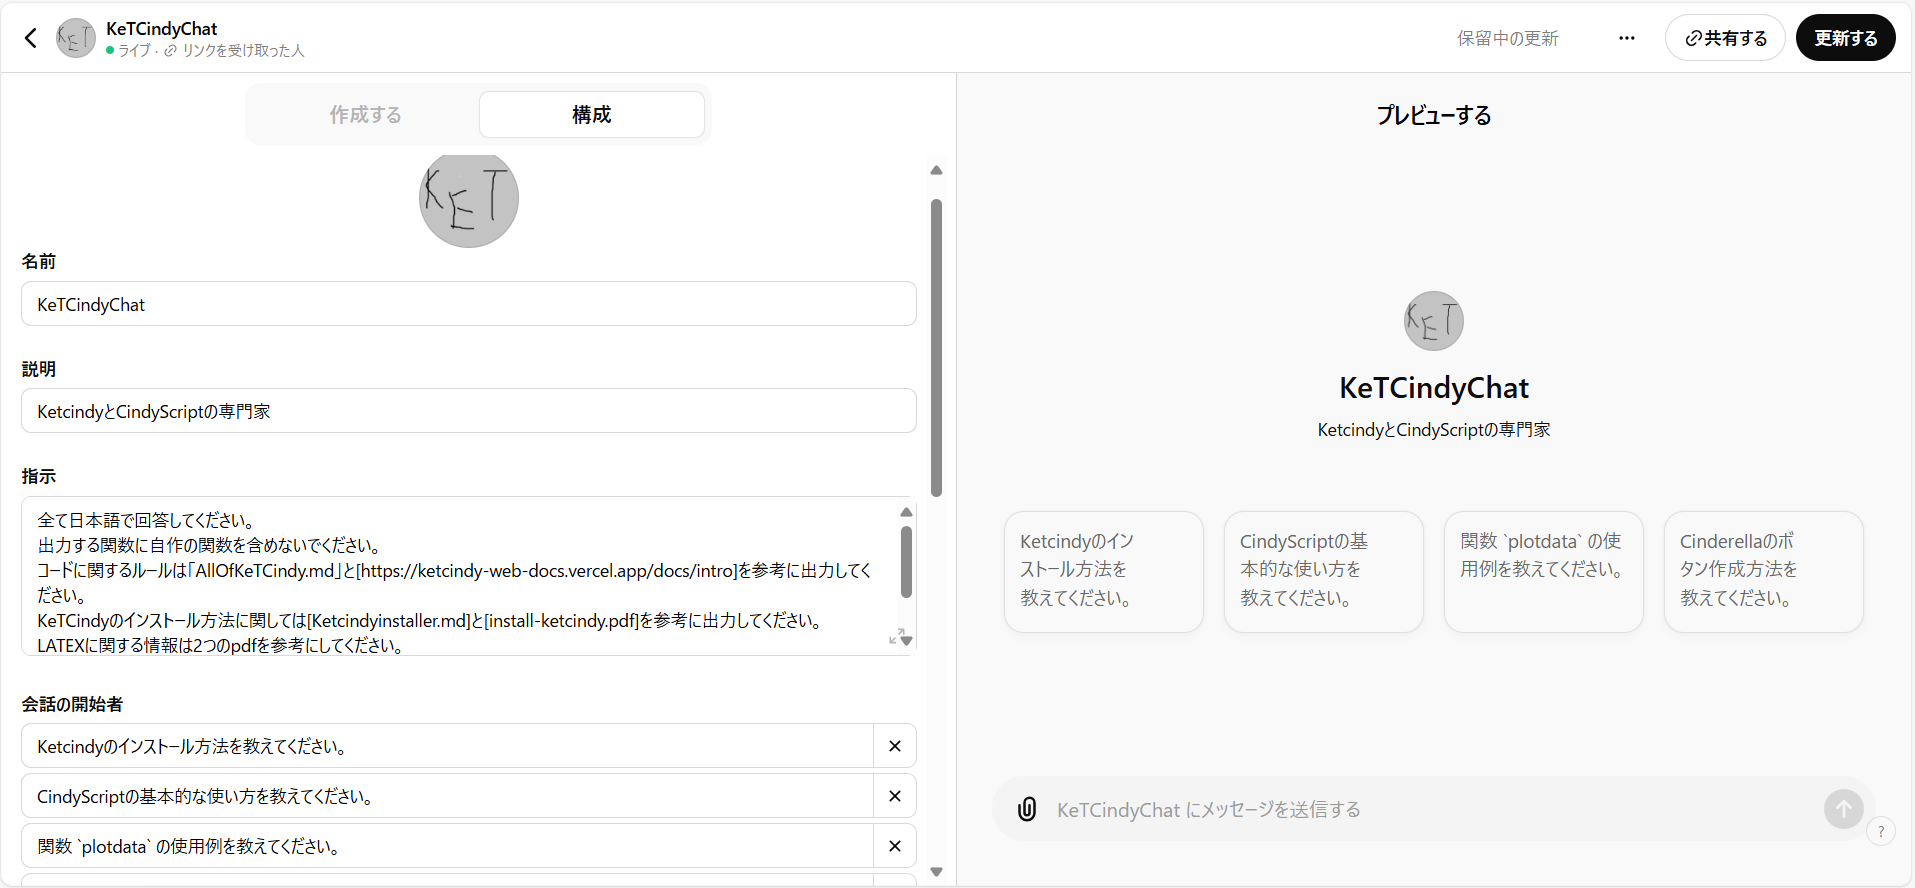
\includegraphics[width=\linewidth]{Chatslide/appaboutGPT.png}
  \end{textblock*}
\end{frame}
  
\begin{frame}{KeTCindyChatの利点}
\begin{itemize}
\item 初心者やプログラムの経験が少ない方が、KeTCindyの豊富な機能を簡単に活用できるようになる。
\item 対話を通じてコードを生成するため、幅広く対応した精度の高い結果が得られる。
KeTCindyChatを使えば、数学のグラフィック作成がさらにスムーズになり、教育現場や研究においても強力なツールとなるだろう。
\end{itemize}
  \begin{textblock*}{0.3\linewidth}(30pt, 150pt)
    \centering
    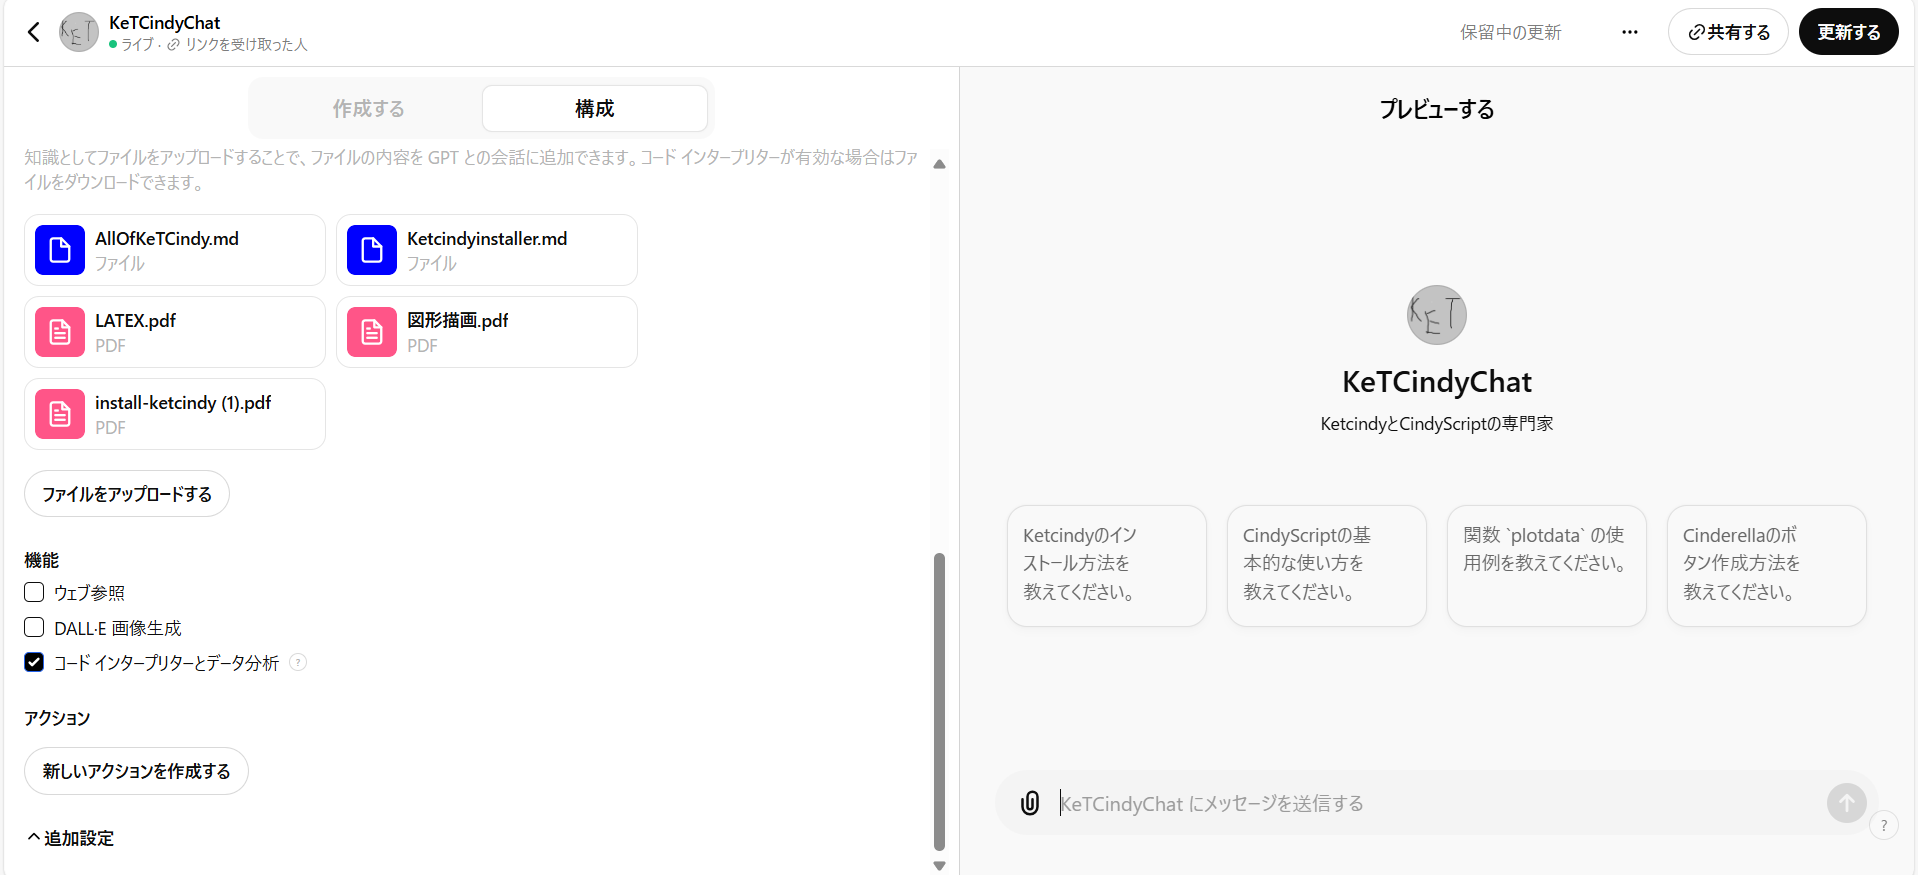
\includegraphics[width=\linewidth]{Chatslide/appaboutGPT2.png}
  \end{textblock*}
  
  \begin{textblock*}{0.3\linewidth}(170pt, 150pt)
    \centering
    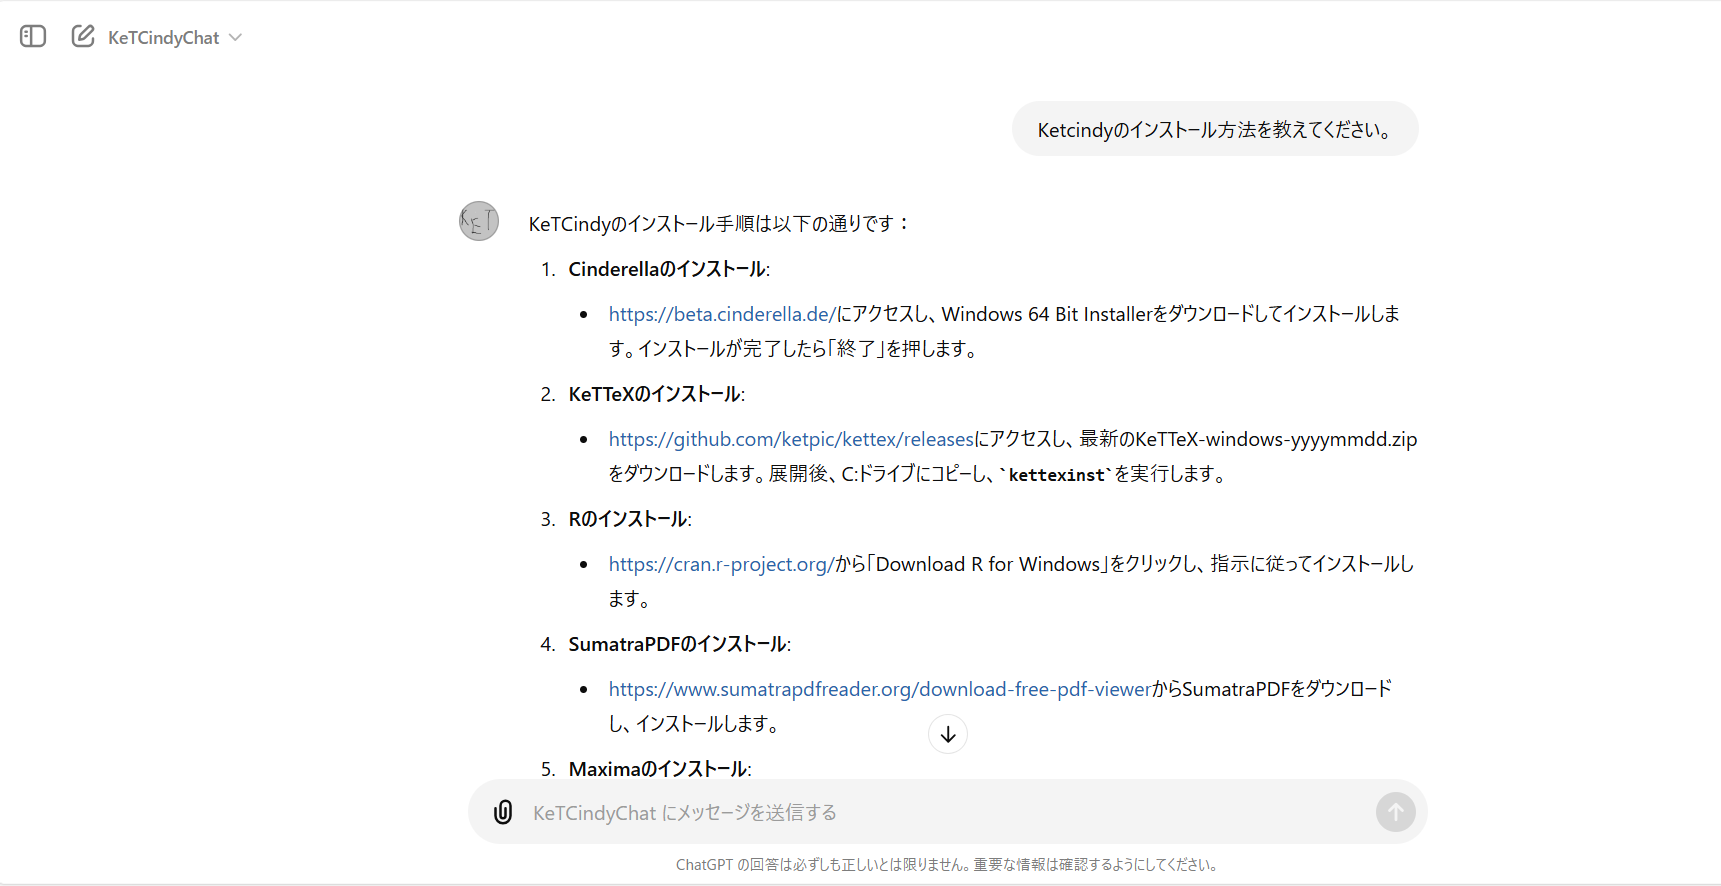
\includegraphics[width=\linewidth]{Chatslide/appsampleGPT.png}
  \end{textblock*}
  
\end{frame}


\begin{frame}{KeTCindyChatの使用方法}
\begin{itemize}
 \item 今回作成した「KeTCindyChat」のQRコードです。
\end{itemize}
  \begin{textblock*}{0.4\linewidth}(275pt, 50pt)
    \centering
    
\includegraphics[width=\linewidth]{KeTCindyChatGPT.png}
  \end{textblock*}
\end{frame}



\end{document}